% =====================================================================
% Cloud Computing Lab: Project8 Report (Question 8)
% IEEE single-column format (IEEEtran, onecolumn)
% Compile with: pdflatex report.tex  (run twice); the cover is cover.tex
% Figures and tables are read from results/ (generated by plot_results.py).
% =====================================================================
\documentclass[journal,onecolumn,12pt]{IEEEtran}

\usepackage[utf8]{inputenc}
\usepackage[T1]{fontenc}
\usepackage{amsmath,amssymb}
\usepackage{graphicx}
\usepackage{booktabs}
\usepackage{array}
\usepackage{tabularx}
\usepackage{threeparttable}
\usepackage{xcolor}
\usepackage{tikz}
\usetikzlibrary{shapes.geometric,arrows.meta,positioning,calc}
\usepackage{algorithm}
\usepackage[noend]{algpseudocode}
\usepackage{listings}
\usepackage{cite}
\usepackage[hidelinks]{hyperref}

% Placeholder macro (red text) so unfinished parts are easy to find
\newcommand{\todo}[1]{\textcolor{red}{[TODO: #1]}}

\definecolor{ink2}{HTML}{52514E}
\lstset{basicstyle=\ttfamily\scriptsize,columns=fixed,keepspaces=true,frame=single,rulecolor=\color{ink2},
        xleftmargin=4pt,xrightmargin=4pt}
\newcommand{\MLB}{M_{\mathrm{LB}}}
\newcommand{\Ubar}{\bar{U}}
% generated table rows: the expandable primitive \@@input is needed inside tabular
\makeatletter\newcommand{\tabinput}[1]{\@@input #1 }\makeatother

\begin{document}

% ---------------- TITLE PAGE ----------------
\title{Implementation and Evaluation of Joint Optimization of Resource Utilization and Makespan in Cloud Computing using a Genetic Algorithm in CloudSim}

\author{Sanskar Shekhar (BTECH/10150/23) and Aman Nautiyal (BTECH/10171/23)\\
Department of Computer Science and Engineering\\
Birla Institute of Technology, Mesra, Ranchi\\
Course: Cloud Computing Lab (IT348) \quad Semester: Seventh}

\markboth{Cloud Computing Lab: Project8 Report}{Shekhar and Nautiyal: GA-based Scheduling in CloudSim}

\maketitle

% ---------------- ABSTRACT ----------------
\begin{abstract}
Task scheduling in cloud data centres must balance two goals: finishing a workload quickly (low makespan) and keeping virtual machines (VMs) busy (high resource utilization, i.e.\ low resource wastage). This report reproduces, in CloudSim 5.0, the core problem studied by Dehury, Kumar and Kumar~\cite{dehury}: assigning independent tasks to heterogeneous VMs with a genetic algorithm (GA) that jointly optimizes makespan and utilization. We formulate the problem, implement the GA on the five-VM configuration assigned in Question 8, and compare it with Round Robin, MCT, Min-Min and Max-Min over 50 to 1000 tasks with 10 paired runs per size. The GA lowers mean makespan by 54.5--57.5\% relative to Round Robin and raises utilization from 57.4--61.1\% to about 99.5\%. In paired tests it is significantly better than MCT up to 200 tasks and than Min-Min up to 500 tasks, but it never beats Max-Min: the two tie up to 200 tasks and Max-Min is better by 0.16--0.21\% at 500 and 1000 tasks, while running 128 to 5\,250 times faster. Further experiments show that (i) the two objectives are almost perfectly aligned in this setting, so the fitness weights barely matter; (ii) the GA's shortfall at 1000 tasks comes from a mutation rate that is too high for long chromosomes, and a rate of $1/n$ closes it; (iii) the paper's own GA, re-implemented exactly from its Algorithm~1, is within about 1\% of Max-Min up to 200 tasks but 9--29\% worse at 500 and 1000 tasks, because its mutation rate of 0.1 and its 100-iteration budget do not scale to long chromosomes; and (iv) modelling each VM as one processing element is accurate for large workloads, whereas giving each VM one processing element per core lengthens small-workload makespans by up to 39\%. The closed-form model and the CloudSim execution agree to within 0.46\% on average (1.37\% at worst).
\end{abstract}

\begin{IEEEkeywords}
Cloud computing, CloudSim, task scheduling, genetic algorithm, makespan, resource utilization, load balancing.
\end{IEEEkeywords}

\section{Introduction}

\IEEEPARstart{C}{loud} data centres execute large numbers of user tasks on shared pools of virtualized resources. How the tasks are mapped to VMs affects both user-facing performance and provider-side efficiency.

\subsection{Background}
Scheduling independent tasks on heterogeneous VMs is NP-hard, so heuristic and metaheuristic methods are widely used. Genetic algorithms~\cite{holland} search the large space of task-to-VM assignments with selection, crossover and mutation and need no problem-specific gradient. Classical list-scheduling heuristics such as Min-Min and Max-Min~\cite{ibarra,braun} give strong baselines at very low cost.

\subsection{Motivation}
A provider wants VMs to be well used (little idle, wasted capacity); a user wants the workload to finish early. A scheduler that optimizes both together is attractive to both, which is the motivation of~\cite{dehury}.

\subsection{Problem Being Addressed}
Given a batch of independent tasks and a set of heterogeneous VMs, find a task-to-VM mapping that jointly minimizes makespan and maximizes resource utilization, following the GA-based approach of Dehury \textit{et al.}~\cite{dehury}, and evaluate it in CloudSim~\cite{cloudsim}.

% ---------------------------------------------------------------------------
\section{Problem Statement and Objectives}

\textit{Problem statement (Question 8).} Design and implement a CloudSim-based simulation that reproduces the core problem addressed in~\cite{dehury}, implement the scheduling approach based on its methodology, design and justify an experimental configuration, evaluate the paper's objectives quantitatively on the VM configuration of Table~\ref{tab:vms}, validate the implementation against the paper, and analyse its behaviour, strengths, limitations and scalability.

\textit{Objectives.}
\begin{enumerate}
\item Formulate the problem: cloud resources, tasks, VMs, decision variables, objectives and constraints (Section~\ref{sec:formulation}).
\item Translate the formulation into a CloudSim simulation (Sections~\ref{sec:arch}--\ref{sec:impl}).
\item Implement a GA scheduler that jointly optimizes makespan and utilization (Section~\ref{sec:ga}).
\item Compare it with Round Robin, Minimum Completion Time (MCT), Min-Min and Max-Min, with paired statistics (Section~\ref{sec:results}).
\item Justify every configuration choice, by argument or by experiment (Sections~\ref{sec:config} and~\ref{sec:extra}).
\item Validate the implementation against the paper and justify each difference (Section~\ref{sec:validation}).
\item Analyse behaviour, strengths, limitations and scalability (Section~\ref{sec:discussion}).
\end{enumerate}

% ---------------------------------------------------------------------------
\section{The Reference Paper and Problem Formulation}\label{sec:formulation}

\subsection{Summary of the Reference Paper}
Dehury, Kumar and Kumar~\cite{dehury} address load balancing in the cloud by scheduling independent tasks on VMs with a genetic algorithm. They treat it as a multi-objective problem with two objectives, \emph{makespan} and \emph{resource wastage}. Resource utilization is the summed task completion time divided by the makespan times the number of VMs, and wastage is one minus utilization. The two objectives are combined by a weighted sum, $f=w_1\cdot\text{Makespan}+w_2\cdot\text{ResW}$, whose weights are left to the application, subject to each task running on one VM and to the CPU and memory capacity of every VM. A solution is an integer vector whose $i$-th gene is the VM of task $i$. The GA (Algorithm~1 of~\cite{dehury}) uses roulette-wheel selection with probability $P_i=(F_{\max}-F_i)/\sum_p(F_{\max}-F_p)$, one-point crossover that turns each pair of parents into two children, per-gene mutation that moves a task to another random VM with probability $m_r$, and $(\mu+\lambda)$ elitist replacement that keeps the best $P$ of parents and children. It is implemented in Python~3.10 on Google Colab and evaluated on the Cloud--Fog Computing task dataset (100--500 tasks) with 60 heterogeneous VMs modelled on nine Amazon EC2 I8g instance types, with a population of 100, 100 iterations and $m_r=0.1$. Compared over 20 runs with Particle Swarm Optimization, Artificial Bee Colony, Black Widow Optimization and random allocation, it reports reductions of up to 16.04\% in makespan and 32.52\% in resource wastage. Table~\ref{tab:corr} (Section~\ref{sec:validation}) compares each element of~\cite{dehury} with our implementation.

\subsection{Problem Elements}
The six elements that Question 8 asks us to identify are:
\begin{itemize}
\item \textbf{Cloud resources:} one data centre with two physical hosts that run the five VMs (Section~\ref{sec:config}).
\item \textbf{Tasks/workload:} a batch of $n$ independent, non-preemptive tasks $T=\{t_1,\dots,t_n\}$ with lengths $L_i$ in million instructions (MI), all available at time 0.
\item \textbf{Virtual machines:} $V=\{v_1,\dots,v_m\}$, $m=5$, with processing capacity $C_j$ (MIPS) derived from the core counts in Table~\ref{tab:vms}.
\item \textbf{Decision variables:} the binary assignment $x_{ij}$ of task $t_i$ to VM $v_j$ (Eq.~\ref{eq:x}).
\item \textbf{Objectives:} minimize makespan $M$ and maximize average utilization $\Ubar$, equivalently minimize resource wastage $1-\Ubar$ (Eqs.~\ref{eq:M}--\ref{eq:F}).
\item \textbf{Constraints:} each task runs on exactly one VM (Eq.~\ref{eq:assign}) and each VM runs its tasks one at a time. In~\cite{dehury} the CPU and memory demands of the tasks placed on a VM must also stay within its capacity; our tasks have no memory demand and each needs one processing element, which every VM provides, so these capacity constraints are always satisfied here.
\end{itemize}

\subsection{Mathematical Formulation}
The expected execution time of task $t_i$ on VM $v_j$ is
\begin{equation}
E_{ij}=\frac{L_i}{C_j}. \label{eq:E}
\end{equation}
The decision variable is
\begin{equation}
x_{ij}=\begin{cases}1 & \text{if task } t_i \text{ is assigned to VM } v_j,\\ 0 & \text{otherwise,}\end{cases}\label{eq:x}
\end{equation}
subject to
\begin{equation}
\sum_{j=1}^{m} x_{ij}=1,\quad \forall i\in\{1,\dots,n\}. \label{eq:assign}
\end{equation}
The busy time (load) of VM $v_j$ and the makespan are
\begin{equation}
B_j=\sum_{i=1}^{n}x_{ij}E_{ij}, \qquad M=\max_{1\le j\le m}B_j. \label{eq:M}
\end{equation}
The average resource utilization, the resource wastage and the degree of imbalance are
\begin{equation}
\Ubar=\frac{1}{m}\sum_{j=1}^{m}\frac{B_j}{M}=\frac{B_{\mathrm{avg}}}{M},\qquad W=1-\Ubar,\qquad
DI=\frac{B_{\max}-B_{\min}}{B_{\mathrm{avg}}}, \label{eq:U}
\end{equation}
where $B_{\mathrm{avg}}$, $B_{\max}$ and $B_{\min}$ are the mean, largest and smallest VM loads. $W$ is the fraction of VM time, up to the makespan, that is left idle. These are exactly the utilization and resource-wastage definitions of~\cite{dehury} (its Eqs.~6 and~7). These definitions reproduce the utilization and imbalance values in the result files: for the 100-task Round Robin run of Fig.~\ref{fig:vmload} the per-VM loads give $\Ubar=0.667$ and $DI=1.057$.

The GA minimizes one fitness value that combines the two objectives:
\begin{equation}
F(x)=w_1\frac{M}{\MLB}+w_2\left(1-\Ubar\right),\qquad \MLB=\frac{\sum_{i=1}^{n}L_i}{\sum_{j=1}^{m}C_j},\qquad w_1=w_2=0.5, \label{eq:F}
\end{equation}
where $\MLB$ is the makespan of a perfectly balanced, perfectly divisible schedule (total work divided by total capacity). It normalizes the makespan term so that both terms are dimensionless. Because $M\ge\MLB$ and $\Ubar\le1$, $F\ge w_1=0.5$. This is a lower bound, not necessarily an attainable value, because tasks cannot be split. The paper~\cite{dehury} uses the same weighted sum with the raw makespan, $f=w_1M+w_2(1-\Ubar)$, and does not fix the weights. In its experiments makespans are of the order of 0.15 (Table~13 of~\cite{dehury}), the same scale as the wastage term. Here makespans range from 24\,s to over 1000\,s, so a raw sum would make the wastage term negligible; dividing by $\MLB$ keeps both terms on the same scale, which preserves the intent of~\cite{dehury} and keeps the weights meaningful.

\textit{Remark on the two objectives.} With these definitions the objectives are closely aligned. A perfectly balanced schedule ($B_j=M$ for all $j$) minimizes both. They can diverge only when work is moved to a slower VM, which raises $B_{\mathrm{avg}}$ (and hence $\Ubar$) without finishing earlier. Section~\ref{sec:weights} measures how much this matters in practice.

% ---------------------------------------------------------------------------
\section{System Architecture and Methodology}\label{sec:arch}

\subsection{Architecture}
Fig.~\ref{fig:arch} shows the simulation. A workload generator creates the cloudlets; each scheduler turns them into a task-to-VM mapping; the broker binds every cloudlet to its VM and CloudSim executes the mapping on the simulated hosts. The same mapping is also evaluated with the closed-form model of Section~\ref{sec:formulation}, which allows the CloudSim execution to be verified (Section~\ref{sec:validation}). Metrics are written to CSV files and processed in Python.

\begin{figure}[!htbp]
\centering
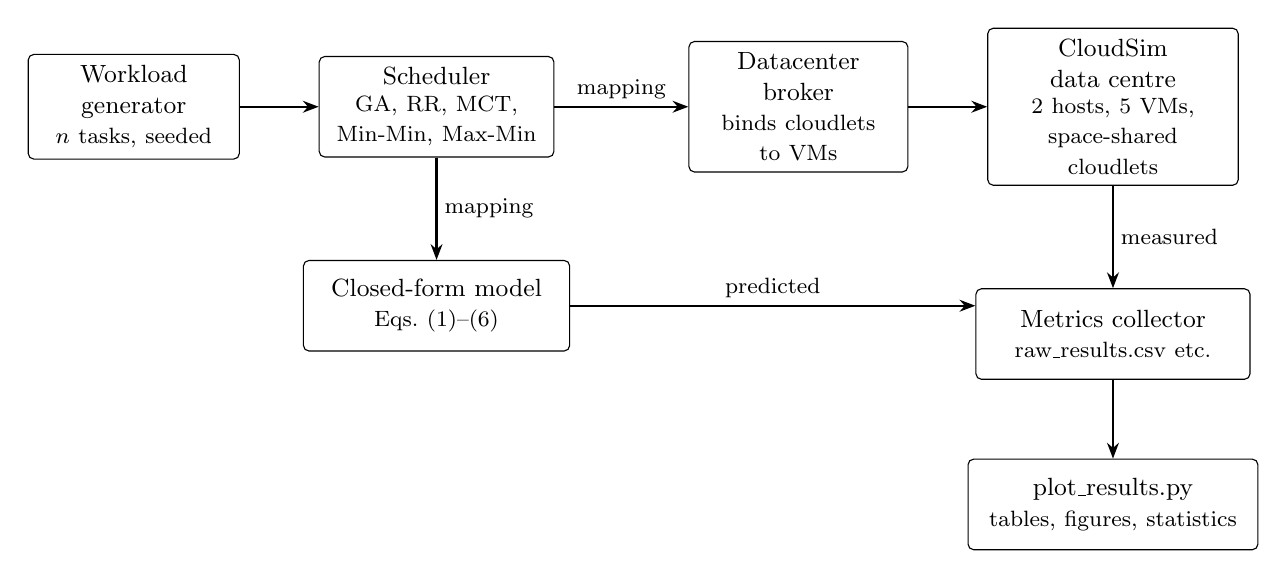
\begin{tikzpicture}[font=\small, box/.style={draw, rounded corners=2pt, align=center, execute at begin node=\hyphenpenalty10000\relax, minimum height=1.15cm, inner sep=4pt},
  arr/.style={-{Stealth[length=2mm]}, thick}, lab/.style={font=\footnotesize, fill=white, inner sep=1.5pt}]
\node[box, text width=2.4cm] (wl) {Workload generator\\ \footnotesize $n$ tasks, seeded};
\node[box, text width=2.7cm, right=1.0cm of wl] (sch) {Scheduler\\ \footnotesize GA, RR, MCT,\\ \footnotesize Min-Min, Max-Min};
\node[box, text width=2.5cm, right=1.7cm of sch] (br) {Datacenter broker\\ \footnotesize binds cloudlets to VMs};
\node[box, text width=2.9cm, right=1.0cm of br] (dc) {CloudSim data centre\\ \footnotesize 2 hosts, 5 VMs,\\ \footnotesize space-shared cloudlets};
\node[box, text width=3.1cm, below=1.3cm of sch] (cf) {Closed-form model\\ \footnotesize Eqs.~(1)--(6)};
\node[box, text width=3.2cm, below=1.3cm of dc] (met) {Metrics collector\\ \footnotesize raw\_results.csv etc.};
\node[box, text width=3.4cm, below=1.0cm of met] (py) {plot\_results.py\\ \footnotesize tables, figures, statistics};
\draw[arr] (wl) -- (sch);
\draw[arr] (sch) -- node[lab, above=1pt]{mapping} (br);
\draw[arr] (br) -- (dc);
\draw[arr] (sch) -- node[lab, right=1pt]{mapping} (cf);
\draw[arr] (cf.east) -- node[lab, above=1pt]{predicted} (cf.east -| met.west);
\draw[arr] (dc) -- node[lab, right=1pt]{measured} (met);
\draw[arr] (met) -- (py);
\end{tikzpicture}
\caption{Architecture of the CloudSim-based simulation.}
\label{fig:arch}
\end{figure}

\subsection{Baseline Schedulers}
\begin{itemize}
\item \textbf{Round Robin (RR):} assigns task $i$ to VM $i \bmod m$, ignoring VM speed.
\item \textbf{MCT:} takes tasks in arrival order and gives each to the VM on which it would complete earliest.
\item \textbf{Min-Min / Max-Min~\cite{ibarra,braun}:} repeatedly compute every unscheduled task's earliest completion time; Min-Min schedules the task with the smallest such time first, Max-Min the task with the largest.
\end{itemize}

\subsection{Genetic Algorithm}\label{sec:ga}
A chromosome is an integer vector of length $n$ whose $i$-th gene is the index of the VM assigned to task $t_i$, so every chromosome satisfies Eq.~(\ref{eq:assign}) by construction. Algorithm~\ref{alg:ga} gives the complete procedure; the parameters are justified in Table~\ref{tab:gaparams}.

\begin{algorithm}[htbp]
\caption{GA-based task scheduling}\label{alg:ga}
\begin{algorithmic}[1]
\State Create a population of $P$ chromosomes with every gene drawn uniformly from $\{1,\dots,m\}$
\For{$g = 1$ \textbf{to} $G$}
  \State Evaluate the fitness $F$ (Eq.~\ref{eq:F}) of every chromosome; update the best chromosome found so far
  \State $\mathit{next} \gets$ copies of the $E=2$ fittest chromosomes \Comment{elitism}
  \While{$|\mathit{next}| < P$}
    \State Select parents $p_1, p_2$, each by a tournament of $k=3$ random chromosomes
    \State With probability $p_c$: $\mathit{child}\gets$ two-point crossover of $p_1,p_2$; otherwise $\mathit{child}\gets p_1$
    \State For each gene, with probability $p_m$, reassign the task to a uniformly random VM
    \State Append $\mathit{child}$ to $\mathit{next}$
  \EndWhile
  \State $\mathit{population}\gets\mathit{next}$
\EndFor
\State \Return the best chromosome found as the task-to-VM mapping
\end{algorithmic}
\end{algorithm}

Each generation therefore contains the two elite chromosomes and $P-2$ new offspring. Two-point crossover copies parent 1 and replaces the genes between two random positions with those of parent 2. For the comparison of Section~\ref{sec:variants}, the GA of~\cite{dehury} is also implemented exactly as given in its Algorithm~1 (class \texttt{PaperGA}), and our GA can seed its initial population with the Max-Min schedule.

\subsection{Workflow}
(1) Create the CloudSim data centre, hosts and VMs; (2) generate the task set; (3) run each scheduler to obtain a mapping and time it; (4) bind the cloudlets to the VMs and run the simulation; (5) record the measured makespan, utilization and imbalance together with the closed-form predictions; (6) repeat for every task count and run; (7) compute tables, figures and paired statistics.

% ---------------------------------------------------------------------------
\section{Experimental Configuration}\label{sec:config}

\subsection{VM Configuration}
Table~\ref{tab:vms} lists the five VMs given in Question 8.

\begin{table}[!htbp]
\caption{Virtual Machine Configuration (Question 8) and Derived Capacity}
\label{tab:vms}
\centering
\begin{tabular}{lcccc}
\toprule
VM & CPU (cores) & RAM (GB) & Bandwidth (Gbps) & Capacity $C_j$ (MIPS) \\
\midrule
VM1 & 4 & 8 & 1.0 & 4000 \\
VM2 & 2 & 4 & 0.5 & 2000 \\
VM3 & 8 & 16 & 2.0 & 8000 \\
VM4 & 6 & 8 & 1.0 & 6000 \\
VM5 & 2 & 8 & 0.5 & 2000 \\
\bottomrule
\end{tabular}
\end{table}

\subsection{Assumptions and Their Justification}
Question 8 and the summary of~\cite{dehury} do not fix the hosts, workload or several modelling details. Table~\ref{tab:assumptions} lists every assumption we made and why.

\begin{table}[!htbp]
\caption{Assumptions and Justification}
\label{tab:assumptions}
\centering
\small
\begin{tabularx}{\textwidth}{@{}>{\raggedright\arraybackslash}p{3.1cm}>{\raggedright\arraybackslash}p{4.2cm}>{\raggedright\arraybackslash}X@{}}
\toprule
Aspect & Choice & Justification \\
\midrule
Core speed & 1000 MIPS per core; $C_j=\text{cores}_j\times1000$ & Gives the VMs the 4:2:8:6:2 capacity ratio implied by Table~\ref{tab:vms}. Only ratios matter: a different per-core speed rescales every time by the same factor and changes no comparison. \\
VM model & Each VM is \emph{one} processing element (PE) of $C_j$ MIPS & Matches $E_{ij}=L_i/C_j$ of the formulation, which treats a VM's capacity as one pool. Its effect is measured in Section~\ref{sec:multipe}: it is small for large workloads and large for small ones. \\
Cloudlet scheduler & Space-shared & Tasks on a VM run one after another, so the VM load is the sum of execution times (Eq.~\ref{eq:M}). \\
RAM and bandwidth & Given to each VM as in Table~\ref{tab:vms}, but not part of the objective & The tasks are compute-bound and carry no data. In CloudSim's default data centre, RAM and bandwidth only constrain where VMs are placed, and a cloudlet's execution time depends on its length and the PE speed. The 300-byte input/output sizes and full utilization models of the cloudlets therefore do not change any result. \\
Hosts & 2 identical hosts, each 32 cores (4 PEs of 8000 MIPS), 64 GB RAM, 20 Gbps, time-shared VM scheduler & Typical dual-socket server size. Their capacity (64 cores, 128 GB) exceeds the 22 cores and 44 GB the VMs need, so placement never constrains the schedule and the study isolates task scheduling, which is the problem of~\cite{dehury}. A PE of 8000 MIPS lets the fastest VM fit on one PE. \\
Workload sizes & 50, 100, 200, 500, 1000 tasks & From 10 to 200 tasks per VM, covering the regime where scheduling decisions matter most (few tasks per VM) to the regime where greedy heuristics are near-optimal. \\
Task lengths & Uniform on $[1000, 20000]$ MI (mean about 10\,500 MI) & A 20:1 spread between the longest and shortest task, so task order matters to list heuristics; execution times range from 0.125\,s to 10\,s. \\
Arrival & All tasks at $t=0$ (batch) & The formulation is a static mapping of a known set of independent tasks. \\
Runs and seeds & 10 runs per size; task set seed $42+1000\cdot\mathit{run}+n$; the GA's random generator uses the same seed & Every scheduler sees the same task set within a run, so results can be compared pairwise (Section~\ref{sec:paired}); the whole experiment is reproducible bit for bit. \\
\bottomrule
\end{tabularx}
\end{table}

\subsection{GA Parameters}
Table~\ref{tab:gaparams} gives the GA parameters. The values sit inside the ranges commonly recommended for GAs~\cite{dejong,grefenstette}, and Section~\ref{sec:sensitivity} tests each one experimentally.

\begin{table}[!htbp]
\caption{Genetic Algorithm Parameters}
\label{tab:gaparams}
\centering
\small
\begin{tabularx}{\textwidth}{@{}>{\raggedright\arraybackslash}p{2.8cm}>{\raggedright\arraybackslash}p{3.5cm}>{\raggedright\arraybackslash}X@{}}
\toprule
Parameter & Value & Justification \\
\midrule
Population $P$ & 100 & Halving it or doubling it changes makespan by at most 0.73 points relative to Max-Min (Table~\ref{tab:sensitivity}); 100 balances quality and run time. \\
Generations $G$ & 300 & Up to 500 tasks the best fitness stops improving by generation 242 or earlier (Fig.~\ref{fig:conv}); at 1000 tasks it is still improving at generation 292, and 100 generations are clearly too few. \\
Initial population & Random, no seeding & A plain GA as in~\cite{dehury}; the seeded hybrid is tested separately (Section~\ref{sec:variants}). \\
Selection & Tournament, $k=3$ & Gives steady selection pressure that does not depend on the scale of $F$~\cite{goldberg}; roulette wheel is compared in Section~\ref{sec:variants}. \\
Crossover & Two-point, $p_c=0.8$ & $p_c$ within the usual 0.6--0.95 range~\cite{dejong,grefenstette}; $p_c=0.6$ and $1.0$ give similar results (Table~\ref{tab:sensitivity}). \\
Mutation & Per-gene random VM, $p_m=0.02$ & Two expected changes per child at 100 tasks. Section~\ref{sec:sensitivity} shows it is too high for 1000-task chromosomes, where $p_m=1/n$~\cite{back} is better; \cite{dehury} uses 0.1. \\
Elitism & Best 2 copied unchanged & Guarantees the best fitness never gets worse; \cite{dehury} achieves the same with $(\mu+\lambda)$ replacement. \\
Fitness weights & $w_1=w_2=0.5$ & Equal priority to the two objectives; the full sweep $w_1\in\{0,\dots,1\}$ is reported in Section~\ref{sec:weights}. \\
\bottomrule
\end{tabularx}
\end{table}

% ---------------------------------------------------------------------------
\section{Implementation}\label{sec:impl}

The simulation is written in Java against the \texttt{org.cloudbus.cloudsim} API of the CloudSim toolkit~\cite{cloudsim}. The results in this report were produced with CloudSim 5.0, the version used in the lab~\cite{panda}; the code also compiles against CloudSim 3.0.3. It has five classes:
\begin{itemize}
\item \texttt{Scheduling}: the closed-form evaluation (loads, makespan, utilization, imbalance, $\MLB$) and the four baseline schedulers.
\item \texttt{GeneticScheduler}: the GA of Algorithm~\ref{alg:ga}, with an option to seed the population with the Max-Min schedule.
\item \texttt{PaperGA}: the GA of~\cite{dehury} exactly as given in its Algorithm~1, used for the comparison in Section~\ref{sec:variants}.
\item \texttt{Q8Main}: builds the data centre, hosts and VMs, generates the cloudlets, runs and times every scheduler, executes each mapping in CloudSim, and writes \texttt{raw\_results.csv} (one row per task count, run and scheduler, with both the predicted and the CloudSim-measured values), \texttt{convergence.csv}, \texttt{vm\_load.csv} and \texttt{environment.txt}.
\item \texttt{Q8Experiments}: the additional studies of Section~\ref{sec:extra} (weight sweep, parameter sensitivity, GA variants and the multi-PE check).
\end{itemize}
The Python script \texttt{plot\_results.py} reads the CSV files with pandas~\cite{pandas}, computes the paired statistics with SciPy~\cite{scipy} and draws the figures with Matplotlib~\cite{matplotlib}. It also writes every table of Sections~\ref{sec:results}--\ref{sec:extra} as a LaTeX file, so the tables in this report are generated directly from the result files. The source code and results are available at \url{https://github.com/shekharsanskar9/Project8}.

% ---------------------------------------------------------------------------
\section{Experimental Setup}\label{sec:setup}

\begin{itemize}
\item \textbf{Hardware:} a virtual machine with 2 vCPUs of an Intel Xeon processor at 2.10\,GHz and 8\,GB of RAM, running Linux 6.18 (x86-64). The scheduling times below were measured on this machine and scale with its speed.
\item \textbf{Software:} CloudSim 5.0 with Apache Commons Math 3.4.1; the code was developed in Eclipse IDE on JDK 8 as prescribed by the lab~\cite{panda}, compiled for Java 8 (\texttt{-source 8 -target 8}) and run on OpenJDK 21.0.12. Analysis with Python 3.13, pandas 3.0.5, SciPy 1.18.1 and Matplotlib 3.11.2.
\item \textbf{Workload and algorithms:} 50, 100, 200, 500 and 1000 tasks on the five VMs of Table~\ref{tab:vms}; Round Robin, MCT, Min-Min, Max-Min and GA.
\item \textbf{Runs:} 10 runs per task count and scheduler (250 CloudSim simulations for the main experiment), plus 950 for the additional studies. Results are reported as mean $\pm$ standard deviation.
\item \textbf{Timing:} before any measurement every scheduler is run on throw-away workloads so that Java's just-in-time compiler has compiled it (warm-up). A GA run is timed directly. The heuristics finish in microseconds, below the timer's useful resolution, so each is called repeatedly for at least 50\,ms and the mean time per call is recorded. Tables report the median over the 10 runs.
\item \textbf{Statistics:} because all schedulers receive the same task set within a run, schedulers are compared on per-run differences: mean difference with a 95\% $t$-confidence interval, the number of runs won, tied and lost, and a two-sided Wilcoxon signed-rank test~\cite{wilcoxon}.
\item \textbf{Metrics:} makespan $M$ (s), makespan relative to the lower bound $M/\MLB$, average utilization $\Ubar$, degree of imbalance $DI$, and scheduling (algorithm execution) time (ms).
\end{itemize}

% ---------------------------------------------------------------------------
\section{Results}\label{sec:results}

\subsection{Main Comparison}
Table~\ref{tab:main} gives the results for every task count. Fig.~\ref{fig:makespan} shows makespan against workload size. Round Robin grows much faster than the other four schedulers, whose curves overlap at this scale. Fig.~\ref{fig:norm} therefore plots makespan divided by the lower bound $\MLB$, which makes the differences between the four visible.

\begin{table}[!htbp]
\caption{Performance Comparison (Mean over 10 Runs)}
\label{tab:main}
\centering
\small
\begin{threeparttable}
\begin{tabular}{rlccccc}
\toprule
Tasks & Scheduler & Makespan (s) & $M/\MLB$ & Util.\ (\%) & Imbalance (DI) & Sched.\ time (ms)\tnote{a} \\
\midrule
\tabinput{results/tables/main_results.tex}
\bottomrule
\end{tabular}
\begin{tablenotes}\footnotesize
\item[a] Median of the 10 runs, measured after JIT warm-up; for the heuristics, the mean of repeated calls lasting at least 50\,ms.
\end{tablenotes}
\end{threeparttable}
\end{table}

\begin{table}[!htbp]
\caption{Paired Makespan Differences (GA minus Baseline, 10 Runs per Size)}
\label{tab:paired}
\centering
\small
\begin{threeparttable}
\begin{tabular}{lrcccc}
\toprule
Comparison & Tasks & Mean diff.\ (s) $\pm$ 95\% CI & Mean diff.\ (\%) & GA wins/ties/losses & Wilcoxon $p$ \\
\midrule
\tabinput{results/tables/paired.tex}
\bottomrule
\end{tabular}
\begin{tablenotes}\footnotesize
\item With 10 pairs the smallest possible two-sided Wilcoxon $p$ is 0.002 (all 10 runs in the same direction).
\end{tablenotes}
\end{threeparttable}
\end{table}

\begin{figure}[!htbp]
\centering
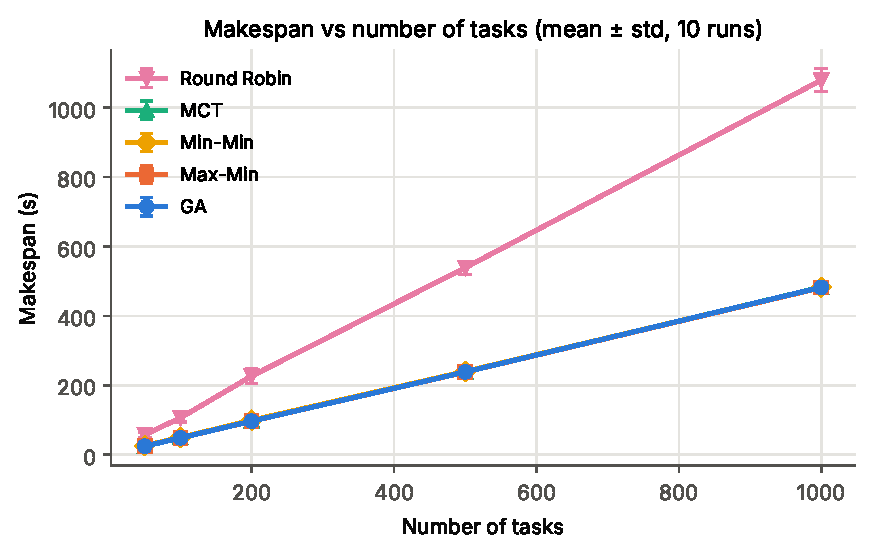
\includegraphics[width=0.72\textwidth]{results/figures/makespan_vs_tasks.pdf}
\caption{Makespan versus number of tasks (mean $\pm$ standard deviation over 10 runs).}
\label{fig:makespan}
\end{figure}

\begin{figure}[!htbp]
\centering
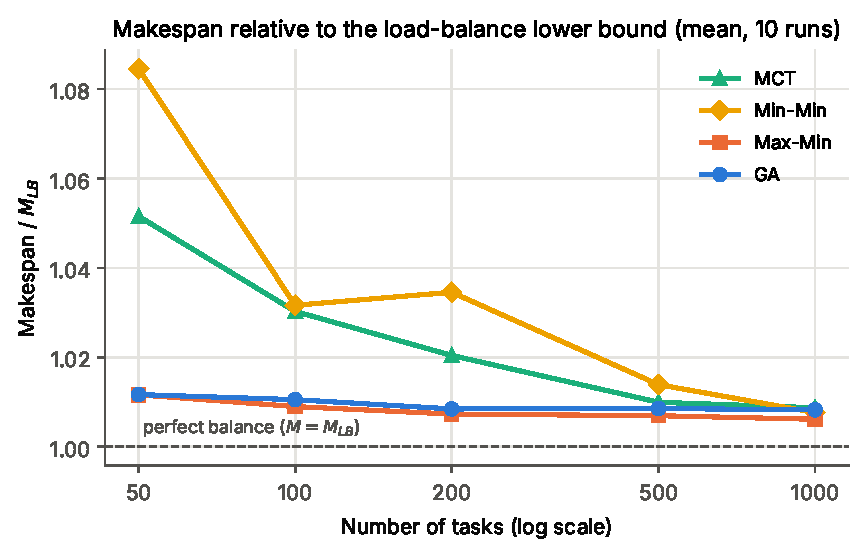
\includegraphics[width=0.72\textwidth]{results/figures/norm_makespan_vs_tasks.pdf}
\caption{Makespan divided by the load-balance lower bound $\MLB$ (mean over 10 runs; Round Robin, at 2.23--2.37, is omitted). The dashed line is a perfectly balanced schedule.}
\label{fig:norm}
\end{figure}

\begin{figure}[!htbp]
\centering
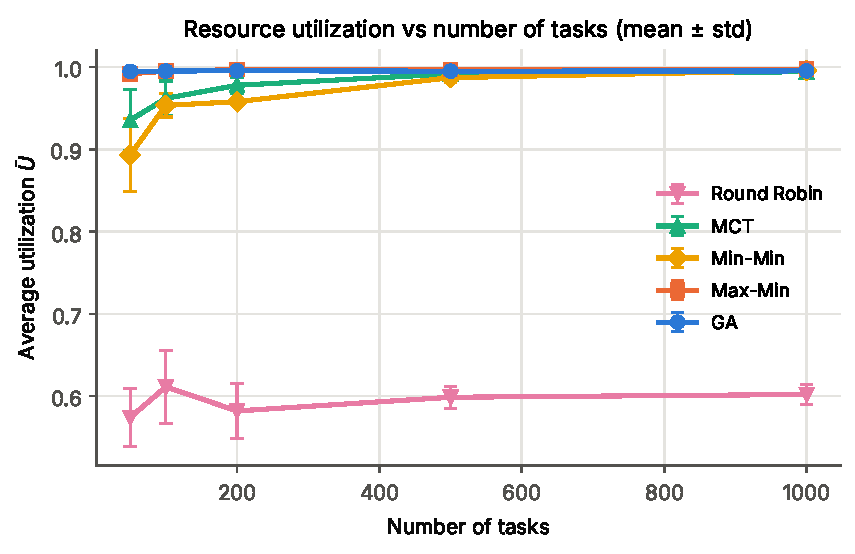
\includegraphics[width=0.72\textwidth]{results/figures/utilization_vs_tasks.pdf}
\caption{Average resource utilization versus number of tasks.}
\label{fig:util}
\end{figure}

\begin{figure}[!htbp]
\centering
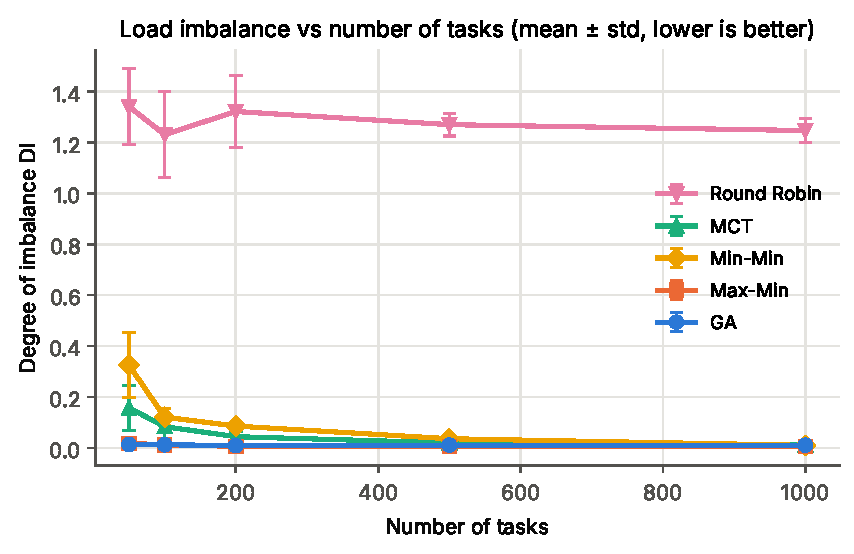
\includegraphics[width=0.72\textwidth]{results/figures/imbalance_vs_tasks.pdf}
\caption{Degree of imbalance versus number of tasks (lower is better).}
\label{fig:imb}
\end{figure}

\begin{figure}[!htbp]
\centering
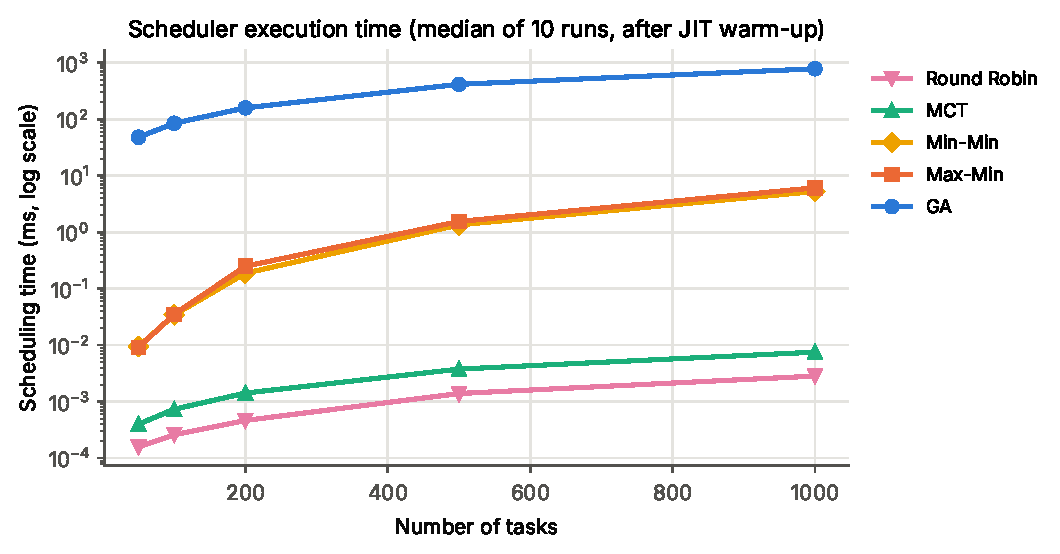
\includegraphics[width=0.78\textwidth]{results/figures/algo_time_vs_tasks.pdf}
\caption{Scheduling (algorithm execution) time versus number of tasks, log scale.}
\label{fig:time}
\end{figure}

\begin{figure}[!htbp]
\centering
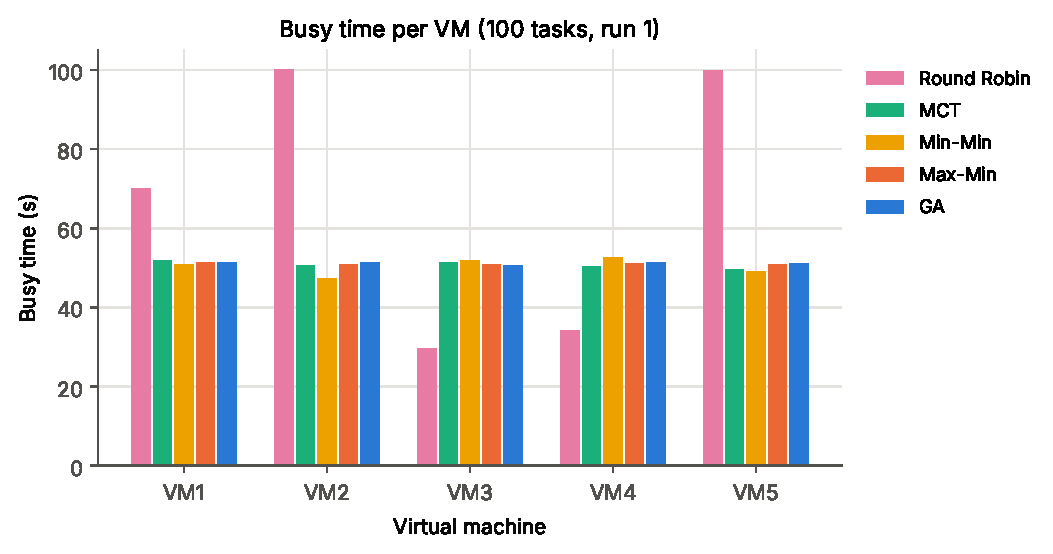
\includegraphics[width=0.78\textwidth]{results/figures/vm_load.pdf}
\caption{Busy time per VM for each scheduler (100 tasks, first run).}
\label{fig:vmload}
\end{figure}

\subsection{Paired Comparison of the GA with the Strong Baselines}\label{sec:paired}
Table~\ref{tab:paired} compares the GA with MCT, Min-Min and Max-Min run by run. A negative difference means the GA finished earlier.


\subsection{GA Convergence}
Fig.~\ref{fig:conv} shows the best fitness in the first run of every task count, plotted as its gap above the bound $F\ge0.5$. In the 100-task run the best fitness falls from 0.872 in generation 1 to below 0.52 by generation 21 and reaches its final value 0.5054 at generation 174, about 1.1\% above the bound. Up to 500 tasks the last improvement comes at generation 242 or earlier. At 1000 tasks the curve is still falling, with its last improvement at generation 292 (final fitness 0.5039): the GA has not converged.

\begin{figure}[!htbp]
\centering
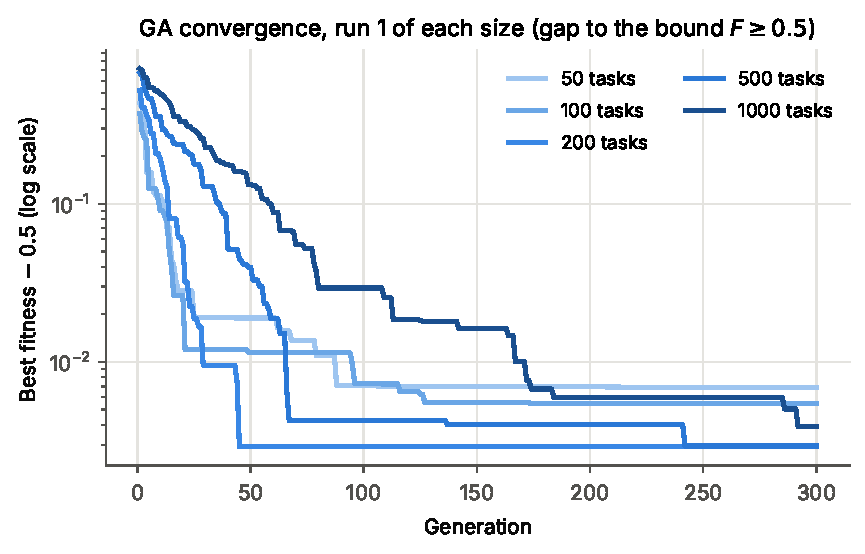
\includegraphics[width=0.72\textwidth]{results/figures/ga_convergence.pdf}
\caption{GA convergence for the first run of each task count; the gap $F-0.5$ to the lower bound is shown on a log scale (lower is better).}
\label{fig:conv}
\end{figure}

\subsection{Console Output}
Fig.~\ref{fig:console} shows the summary that \texttt{Q8Main} prints at the end of the run that produced Table~\ref{tab:main}. The printed scheduling times are means over the 10 runs; Table~\ref{tab:main} reports medians.

\begin{figure}[!htbp]
\centering
\begin{minipage}{0.92\textwidth}
\lstinputlisting[basicstyle=\ttfamily\scriptsize,breaklines=true,breakatwhitespace=true]{results/console.txt}
\end{minipage}
\caption{Console output of \texttt{Q8Main} for the reported run.}
\label{fig:console}
\end{figure}

% ---------------------------------------------------------------------------
\section{Additional Experiments}\label{sec:extra}

\subsection{Fitness Weights: Is There a Trade-off?}\label{sec:weights}
To test whether the two objectives actually compete, the GA was run with $w_1\in\{0, 0.25, 0.5, 0.75, 1\}$ and $w_2=1-w_1$ on the same task sets (100 and 500 tasks, 10 runs each). Table~\ref{tab:weights} and Fig.~\ref{fig:weights} show the result. The last column is the total VM busy time divided by its minimum possible value $m\,\MLB$; it would rise above 1 if the GA shifted work to slower VMs to raise utilization.

\begin{table}[!htbp]
\caption{Effect of the Fitness Weights (GA, Mean over 10 Runs)}
\label{tab:weights}
\centering
\small
\begin{tabular}{rcccccccc}
\toprule
Tasks & $w_1$ & $w_2$ & Makespan (s) & $M/\MLB$ & Util.\ (\%) & DI & Busy time / $m\MLB$ \\
\midrule
\tabinput{results/tables/weights.tex}
\bottomrule
\end{tabular}
\end{table}

\begin{figure}[!htbp]
\centering
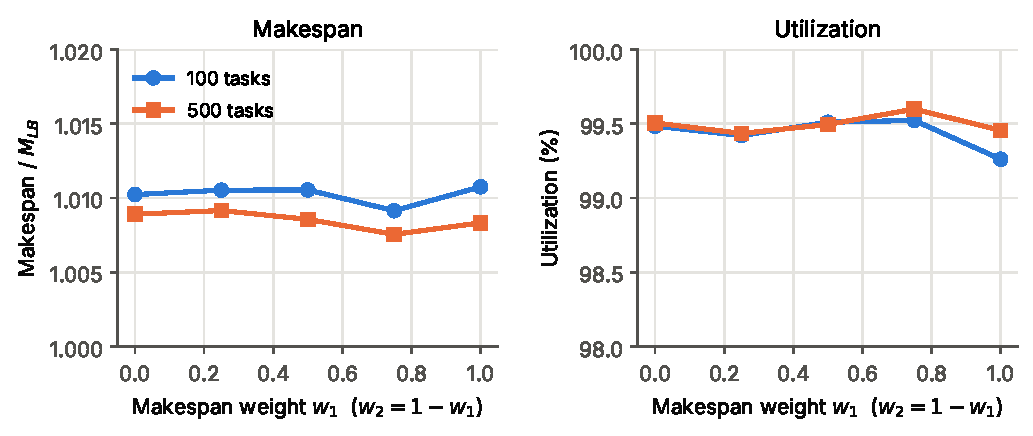
\includegraphics[width=0.86\textwidth]{results/figures/weights.pdf}
\caption{Makespan (relative to $\MLB$) and utilization of the GA for different fitness weights (mean of 10 runs). The axes span 2\% so that the small size of the effect is visible.}
\label{fig:weights}
\end{figure}

Across the whole sweep the mean makespan changes by less than 0.2\% (48.20--48.28\,s at 100 tasks, 238.15--238.53\,s at 500 tasks) and utilization stays between 99.26\% and 99.60\%. Total busy time stays within 0.6\% of its minimum for every weight, including $w_1=0$, where the fitness rewards only utilization: the GA does not raise utilization by shifting work to slower VMs. The highest utilization and lowest makespan come at the same weight ($w_1=0.75$ for both sizes), so the objectives do not trade off: in this setting optimizing either one optimizes the other.

\subsection{GA Parameter Sensitivity}\label{sec:sensitivity}
Each GA parameter was varied one at a time around the default on the same 10 task sets for 100 and 1000 tasks. Table~\ref{tab:sensitivity} reports $M/\MLB$, the mean makespan difference from Max-Min on the same task set, the number of runs in which the GA beat Max-Min, and the median scheduling time. The default is $P=100$, $G=300$, $p_c=0.8$, $p_m=0.02$.

\begin{table}[!htbp]
\caption{GA Parameter Sensitivity (One Factor at a Time, 10 Runs)}
\label{tab:sensitivity}
\centering
\footnotesize
\setlength{\tabcolsep}{4pt}
\begin{threeparttable}
\begin{tabular}{lcccc|cccc}
\toprule
 & \multicolumn{4}{c|}{100 tasks} & \multicolumn{4}{c}{1000 tasks} \\
Setting & $M/\MLB$ & $\Delta$MM (\%) & beats & ms & $M/\MLB$ & $\Delta$MM (\%) & beats & ms \\
\midrule
\tabinput{results/tables/sensitivity.tex}
\bottomrule
\end{tabular}
\begin{tablenotes}\footnotesize
\item $\Delta$MM: mean makespan difference from Max-Min on the same task set (negative = GA better); beats: runs in which the GA's makespan is below Max-Min's; ms: median scheduling time.
\end{tablenotes}
\end{threeparttable}
\end{table}

At 100 tasks no setting moves the GA more than 0.41\% from Max-Min, and several settings (population 50, 1000 generations) beat it slightly on average. At 1000 tasks the mutation rate dominates. With $p_m=0.02$ a 1000-gene child receives about 20 random reassignments; near a balanced schedule almost every such change makes balance worse, so most offspring are worse than their parents. With $p_m=1/n$ (one expected change per child, the classic recommendation~\cite{back}) or $p_m=0.005$, the GA closes the gap to Max-Min ($-0.01\%$ and $+0.03\%$), while $p_m=0.05$ is 15.87\% worse. A budget of 100 generations is far too small at 1000 tasks (+6.72\%). The main results keep the default parameters so that all experiments are consistent, but $p_m=1/n$ is the better choice for large workloads.

\subsection{The Paper's GA and a Seeded Hybrid}\label{sec:variants}
Two further GAs were run on all task sets. The first is the GA of~\cite{dehury} implemented exactly as its Algorithm~1 (class \texttt{PaperGA}): roulette-wheel selection with $P_i\propto F_{\max}-F_i$, one-point crossover producing two children per pair, per-gene mutation and $(\mu+\lambda)$ replacement, with the paper's settings of $P=100$, 100 iterations and $m_r=0.1$. To separate the effect of the mutation rate it was also run with $m_r=1/n$. Both use the fitness of Eq.~(\ref{eq:F}), so only the algorithm differs from ours. The second is our GA with one initial chromosome set to the Max-Min schedule. Table~\ref{tab:variants} and Fig.~\ref{fig:variants} show the results.

\begin{table}[!htbp]
\caption{GA Variants Compared with Max-Min (Mean over 10 Runs)}
\label{tab:variants}
\centering
\footnotesize
\setlength{\tabcolsep}{4pt}
\begin{tabular}{rlcccccc}
\toprule
Tasks & Variant & Makespan (s) & $M/\MLB$ & Util.\ (\%) & vs Max-Min (\%) & W/T/L & ms \\
\midrule
\tabinput{results/tables/variants.tex}
\bottomrule
\end{tabular}
\end{table}

\begin{figure}[!htbp]
\centering
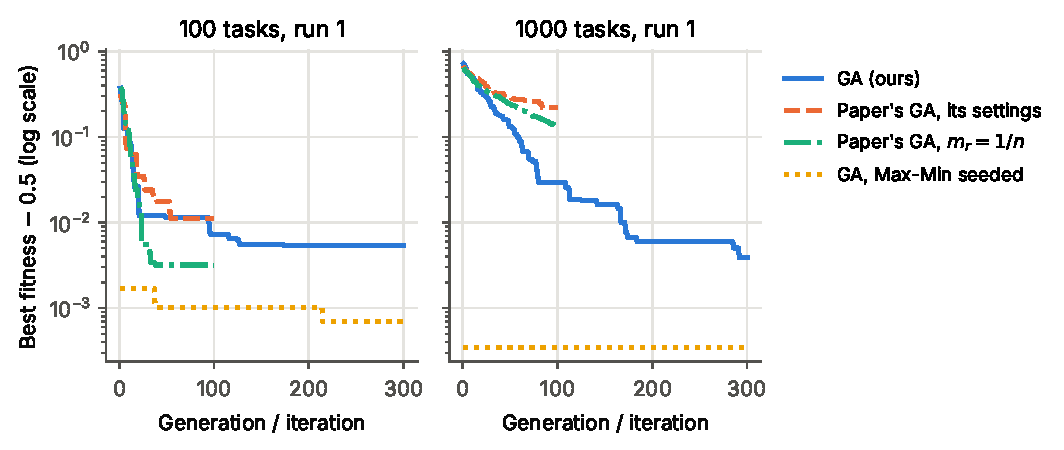
\includegraphics[width=0.92\textwidth]{results/figures/ga_variants_convergence.pdf}
\caption{Convergence of the GA variants in the first run with 100 and 1000 tasks (gap to the bound $F\ge0.5$, log scale). The paper's GA runs for its 100 iterations.}
\label{fig:variants}
\end{figure}

With its own settings the paper's GA is 0.98--1.13\% worse than Max-Min at 50--200 tasks, the range of workloads it was designed for, and falls far behind at 500 and 1000 tasks (9.22\% and 29.37\% worse, with utilization down to 85.7\%). The convergence curves show why. At 1000 tasks a mutation rate of 0.1 changes about 100 genes of every child, so almost every child is worse than its parents and the $(\mu+\lambda)$ step discards it: the best fitness does not change between iteration 90 and 100 (0.7207). With $m_r=1/n$ the paper's GA matches ours at 100 and 200 tasks (0.14\% from Max-Min) in about a third of the time (28\,ms against 85\,ms at 100 tasks), and at 1000 tasks it is still improving at iteration 100, so there the 100-iteration budget is the limit (18.95\% worse). Its selection scheme is not the cause: probabilities proportional to $F_{\max}-F_i$ give the worst chromosome no chance and put strong pressure on the best. What matters is the mutation rate and the iteration budget, which~\cite{dehury} sets for 100--500 tasks spread over 60 VMs (fewer than 10 tasks per VM), whereas here each VM receives 10 to 200 tasks.

The Max-Min-seeded GA is never worse than Max-Min by more than 0.07\% on average, and at 500 and 1000 tasks its result has exactly the fitness and makespan of the Max-Min seed in all 20 runs: within 300 generations the GA could not improve on it. At 50--200 tasks it found schedules with a lower closed-form fitness than Max-Min in 21 of 30 runs; in 15 of these, CloudSim measured a slightly \emph{longer} makespan (by 0.17\% on average). Differences this small are below the 0.46\% average gap between the closed-form model and CloudSim (Section~\ref{sec:verify}), so they should not be read as real wins or losses.

\subsection{Effect of Modelling a VM as One Processing Element}\label{sec:multipe}
To quantify the single-PE assumption of Table~\ref{tab:assumptions}, every mapping of the main experiment was executed a second time with each VM modelled as $\text{cores}_j$ PEs of 1000\,MIPS (hosts of 32 PEs of 1000 MIPS), so that a $c$-core VM runs up to $c$ tasks in parallel. Table~\ref{tab:multipe} gives the change in CloudSim makespan.

\begin{table}[!htbp]
\caption{Makespan Change When VMs Have One PE per Core (\%, Mean over 10 Runs)}
\label{tab:multipe}
\centering
\small
\begin{tabular}{rccccc}
\toprule
Tasks & Round Robin & MCT & Min-Min & Max-Min & GA \\
\midrule
\tabinput{results/tables/multipe.tex}
\bottomrule
\end{tabular}
\end{table}

With one PE per core, a task can use only one core's speed: a 20\,000\,MI task takes 20\,s on any VM instead of 2.5\,s on VM3. With few tasks per core the last long tasks then finish late, so makespan grows by 29.5--38.6\% at 50 tasks for the four load-balancing schedulers. The effect shrinks as the number of tasks per core grows (1.3--1.6\% at 1000 tasks). The single-PE model is the one that matches the formulation of~\cite{dehury} and is accurate for large workloads, but at small workloads absolute makespans depend on it. The ranking of the four load-balancing schedulers also changes under the multi-PE model at every size except 100 tasks, while Round Robin stays last everywhere. Differences of a few tenths of a percent between the GA, Max-Min, Min-Min and MCT are therefore model-dependent.

% ---------------------------------------------------------------------------
\section{Validation}\label{sec:validation}

\subsection{Verification of the CloudSim Model Against the Formulation}\label{sec:verify}
Every mapping is evaluated twice: with the closed-form model of Section~\ref{sec:formulation} and by executing it in CloudSim. Over all 250 runs of the main experiment the CloudSim makespan differs from the formula by 0.46\% on average and 1.37\% at most, and it is the higher of the two in 95\% of runs, because the simulator's event processing adds small delays; utilization differs by at most 0.0066. For the 100-task Round Robin run, the per-VM busy times of Fig.~\ref{fig:vmload} also reproduce the reported utilization (0.667) and imbalance (1.057). This confirms that the simulation implements the formulation: independent tasks, each assigned to exactly one VM, VM load equal to the sum of task execution times, and makespan equal to the largest load.

\subsection{Correspondence with the Reference Paper}
Table~\ref{tab:corr} compares each element of~\cite{dehury} with our implementation and justifies every difference.

\begin{table}[!htbp]
\caption{Correspondence Between the Paper and This Implementation}
\label{tab:corr}
\centering
\small
\begin{threeparttable}
\begin{tabularx}{\textwidth}{@{}>{\raggedright\arraybackslash}p{2.1cm}>{\raggedright\arraybackslash}p{3.6cm}>{\raggedright\arraybackslash}p{3.6cm}>{\raggedright\arraybackslash}X@{}}
\toprule
Element & Paper~\cite{dehury} & This implementation & Same? / justification \\
\midrule
Problem & Load balancing: independent tasks on VMs, each task on one VM & Batch of independent tasks on the 5 VMs of Question~8 & Same. \\
Objectives & Makespan and resource wastage $1-U_{VM}$ (Eqs.~5--7 of~\cite{dehury}) & $M$ and $W=1-\Ubar$ (Eqs.~\ref{eq:M}--\ref{eq:U}) & Same definitions. \\
Fitness & $w_1\cdot\text{Makespan}+w_2\cdot\text{ResW}$; weights not fixed & $w_1M/\MLB+w_2W$, $w_1=w_2=0.5$ & Makespan normalized so both terms have the same scale (Section~\ref{sec:formulation}-C); weights shown not to matter here (Section~\ref{sec:weights}). \\
Constraints & One VM per task; CPU and memory capacity of each VM & One VM per task; capacity always satisfied & Tasks have no memory demand and need one PE each (Table~\ref{tab:assumptions}). \\
Encoding & Integer vector, gene $i$ = VM of task $i$ & Same & Same. \\
Initial population & Random & Random & Same. \\
Selection & Roulette wheel, $P_i\propto F_{\max}-F_i$ & Tournament, $k=3$ & Different. The paper's GA is reproduced exactly in Section~\ref{sec:variants}; its gap comes from the mutation rate and budget, not from selection. \\
Crossover & One-point, two children per pair, always applied & Two-point, one child, $p_c=0.8$ & Different; included in the reproduction of Section~\ref{sec:variants}. \\
Mutation & Per-gene move to another random VM, $m_r=0.1$ & Per-gene random VM, $p_m=0.02$ & Same operator. A rate of 0.1 is too high for long chromosomes here (Sections~\ref{sec:sensitivity} and~\ref{sec:variants}). \\
Replacement & $(\mu+\lambda)$: best $P$ of parents and children & Generational, best 2 kept & Both elitist: the best fitness never gets worse. \\
GA parameters & $P=100$, 100 iterations, $m_r=0.1$ & $P=100$, $G=300$, $p_c=0.8$, $p_m=0.02$ & More generations because our largest workload has 1000 tasks (Table~\ref{tab:gaparams}, Section~\ref{sec:sensitivity}). \\
Environment & Cloud--Fog task dataset (100--500 tasks); 60 VMs of 9 AWS EC2 I8g types, 105 MIPS per vCPU & The 5 VMs of Question~8; seeded synthetic tasks, 50--1000 & VMs fixed by Question~8; a seeded synthetic workload keeps the study reproducible (Table~\ref{tab:assumptions}). \\
Simulator & Own Python~3.10 simulation on Google Colab & CloudSim 5.0 (Java) & Required by Question~8. \\
Baselines & PSO, ABC, BWO, random allocation & RR, MCT, Min-Min, Max-Min & Classic heuristics, including strong list schedulers; metaheuristic baselines are left for future work. \\
Runs and statistics & 20 independent runs, ANOVA & 10 paired runs, Wilcoxon signed-rank test & Paired design: all schedulers see the same task sets. \\
Metrics & Makespan, resource wastage, fitness, degree of imbalance, task completion time & Makespan, $\Ubar$ and $W$, DI, scheduling time & Covers both objectives of~\cite{dehury}. \\
\bottomrule
\end{tabularx}
\end{threeparttable}
\end{table}

\subsection{Comparison with the Paper's Results}
The study in~\cite{dehury} uses different data, 60 VMs and different baselines (Table~\ref{tab:corr}), so its numbers cannot be reproduced directly; the comparison is qualitative.

\textit{Where the results agree.} Like~\cite{dehury}, the GA strongly improves on a naive allocation. In~\cite{dehury} it lowers the makespan at 500 tasks from 0.91 under random allocation to 0.69, and resource wastage from about 0.38--0.60 to 0.22--0.40. Here, against Round Robin, it cuts makespan by 54.5--57.5\% and wastage $W$ from about 39--43\% of VM time to about 0.5\%. In both studies imbalance falls as the number of tasks grows (Fig.~\ref{fig:imb} for MCT and Min-Min; Fig.~12 of~\cite{dehury}), because many small tasks can be spread more evenly than a few large ones.

\textit{Where they differ.} In~\cite{dehury} the GA is best in fitness and makespan among the metaheuristics compared (ANOVA, $p<0.0001$), but the paper's own ANOVA finds no significant difference in resource wastage ($p=0.063$; ABC has the lowest mean). Here, too, the GA has no advantage over the strongest competitor: it ties Max-Min up to 200 tasks and loses by 0.16--0.21\% at 500 and 1000 tasks (9 of 10 runs, $p=0.004$); under the closed-form model Max-Min wins every run from 200 tasks upward. Max-Min is a strong list heuristic that already ends less than 1.2\% above the lower bound on this five-VM problem, and~\cite{dehury} does not compare against it. The wastage reached in~\cite{dehury} (0.22--0.41) is much higher than here (about 0.005) because with fewer than 10 tasks per VM a schedule cannot be balanced finely, whereas here every VM receives 10 to 200 tasks. Finally, the paper's GA with its own settings is about 1\% behind Max-Min at the workload sizes it was designed for and falls further behind at larger sizes (Section~\ref{sec:variants}), so its parameters need to be scaled with the number of tasks.

% ---------------------------------------------------------------------------
\section{Analysis and Discussion}\label{sec:discussion}

\subsection{What Worked}
\textit{Makespan.} The GA lowers mean makespan by 57.5\%, 54.5\%, 57.4\%, 55.8\% and 55.3\% relative to Round Robin for 50, 100, 200, 500 and 1000 tasks (Table~\ref{tab:main}). Round Robin ignores VM speed, so the slow two-core VMs receive as many tasks as the eight-core VM. Fig.~\ref{fig:vmload} shows the consequence: for 100 tasks the Round Robin loads range from 29.5\,s (VM3) to 100.1\,s (VM2), whereas every other scheduler keeps all five VMs between 47.2\,s and 52.5\,s.

\textit{Utilization and imbalance.} The GA keeps utilization at 99.5\% for every workload size, against 57.4--61.1\% for Round Robin (Fig.~\ref{fig:util}), and its degree of imbalance stays between 0.009 and 0.014, against 1.23--1.34 (Fig.~\ref{fig:imb}).

\textit{Against MCT and Min-Min.} The GA is significantly faster-finishing than MCT at 50, 100 and 200 tasks (3.75\%, 1.90\% and 1.17\% lower makespan; 10, 10 and 9 of 10 runs) and than Min-Min at 50 to 500 tasks (6.68\% down to 0.53\%; 10 of 10 runs at every size). At 1000 tasks neither difference is significant.

\subsection{What Did Not Work}
\textit{Against Max-Min.} The GA does not outperform Max-Min at any size. The difference is not significant up to 200 tasks, and Max-Min is better at 500 and 1000 tasks (Table~\ref{tab:paired}). Seeding the GA with the Max-Min schedule makes it at least as good as Max-Min but no better at 500 and 1000 tasks (Table~\ref{tab:variants}).

\textit{Convergence at 1000 tasks.} With the default $p_m=0.02$ the GA is still improving at generation 292 of 300 (Fig.~\ref{fig:conv}). Section~\ref{sec:sensitivity} shows the cause is the mutation rate, not only the generation budget: $p_m=1/n$ matches Max-Min within 0.01\% at the same cost.

\textit{Cost.} The GA takes a median of 48\,ms for 50 tasks and 784\,ms for 1000 tasks, against 0.009\,ms and 6.1\,ms for Max-Min. It is therefore 128 to 5\,250 times slower (Fig.~\ref{fig:time}). In absolute terms this is small: 784\,ms is 0.16\% of the 482\,s makespan it schedules, and the overhead stays below 0.2\% of the makespan at every size. For a batch scheduler this cost is acceptable; it would matter only for very frequent rescheduling or much larger problems.

\subsection{Why the Results Look This Way}
With only five VMs and tens to hundreds of tasks per VM, a greedy completion-time heuristic already places work almost perfectly: Max-Min schedules the longest tasks first and fills the gaps with short ones, ending less than 1.2\% above the lower bound at every size (Fig.~\ref{fig:norm}). Utilization cannot exceed 100\%, so the remaining room for any scheduler is under about 1\%. MCT and Min-Min make early placement mistakes that matter when there are few tasks per VM, which is why the GA's advantage over them is largest at 50 tasks and fades as the workload grows. The weight sweep (Section~\ref{sec:weights}) shows why the joint objective behaves like a single one here: a balanced schedule maximizes utilization and minimizes makespan at the same time.

\subsection{Trends}
All load-balancing schedulers approach the lower bound as the workload grows ($M/\MLB$ falls from 1.012--1.085 at 50 tasks to 1.006--1.009 at 1000 tasks); Round Robin stays at 2.23--2.37 times the bound. The heuristics' scheduling time grows roughly quadratically for Min-Min and Max-Min and linearly for MCT and Round Robin, while the GA's grows linearly with the number of tasks (its cost per generation is proportional to $P\cdot n$).

\subsection{Strengths}
The GA gives near-perfect balance (utilization about 99.5\%, DI about 0.01) at every size, beats MCT and Min-Min on small and medium workloads, and its fitness function can be extended with further objectives (energy, cost, deadlines) without changing the algorithm, which a list heuristic cannot do.

\subsection{Limitations}
\begin{enumerate}
\item The GA never clearly beats Max-Min, and its advantage over MCT and Min-Min disappears at 1000 tasks.
\item Its scheduling time is two to three orders of magnitude higher than the heuristics', although under 0.2\% of the makespan.
\item The experiments use five VMs, independent tasks and one synthetic workload family, so the conclusions may not hold for larger or more heterogeneous clusters, real traces or dependent-task workflows.
\item Absolute makespans at small workloads depend on the single-PE VM model, and the order of the four load-balancing schedulers changes under the multi-PE model (Section~\ref{sec:multipe}).
\item With 10 runs per setting, differences below about 0.2\% are within the run-to-run variation and the 0.46\% average model-to-simulator gap, and should not be over-interpreted; the paired tests in Table~\ref{tab:paired} mark which differences are significant.
\item Scheduling times were measured on one 2-vCPU machine; the ratios between schedulers are more reliable than the absolute values.
\end{enumerate}

\subsection{Scalability}
Makespan grows linearly with the number of tasks for all schedulers: about 0.48\,s per task for the GA (and MCT, Min-Min and Max-Min) at every size, against 1.06--1.15\,s for Round Robin. The GA's scheduling time grows from 48\,ms to 784\,ms for a 20-fold increase in tasks (16-fold), but a fixed budget of 300 generations becomes insufficient for long chromosomes unless the mutation rate is scaled as $1/n$. Max-Min's time grows faster (from 0.009 to 6.1\,ms, about 670-fold), so the cost ratio narrows from about 5\,250 to 128 as the workload grows.

% ---------------------------------------------------------------------------
\section{Conclusion}
We reproduced the joint makespan and utilization optimization problem of~\cite{dehury} in CloudSim 5.0 and compared a GA scheduler with Round Robin, MCT, Min-Min and Max-Min on 50 to 1000 tasks with paired runs. The GA cut makespan by 54.5--57.5\% and raised utilization from about 60\% to 99.5\% relative to Round Robin, and it was significantly better than MCT up to 200 tasks and than Min-Min up to 500 tasks. It did not beat Max-Min: they tie up to 200 tasks and Max-Min is 0.16--0.21\% better at 500 and 1000 tasks while being 128 to 5\,250 times cheaper to compute. In this setting the two objectives are aligned rather than competing; the GA's large-workload shortfall is caused by its mutation rate and disappears with $p_m=1/n$; and the paper's own GA, reproduced exactly, is about 1\% behind Max-Min up to 200 tasks and 9--29\% behind at 500--1000 tasks because its mutation rate and iteration budget do not scale with the number of tasks. The closed-form model matched CloudSim to within 1.37\% in every run. The GA's main benefit here is therefore flexibility, not raw performance.

% ---------------------------------------------------------------------------
\section{Future Scope}
\begin{itemize}
\item Use $p_m=1/n$ and a convergence-based stopping rule instead of a fixed generation count.
\item Seed the population with Max-Min and add a local-search step (e.g.\ swapping tasks between the most and least loaded VMs), which can improve on a seed that plain crossover and mutation cannot.
\item Add objectives that do conflict with makespan, such as energy, monetary cost or SLA deadlines, where a GA's flexibility pays off, and use a Pareto method (e.g.\ NSGA-II).
\item Compare with the metaheuristics used in~\cite{dehury} (PSO, ABC, BWO) and evaluate on real workload traces and larger, more heterogeneous VM pools.
\item Extend to dependent-task workflows and to multi-PE VMs with a matching formulation.
\end{itemize}

% ---------------------------------------------------------------------------
% ---------------- REFERENCES ----------------
\begin{thebibliography}{99}

\bibitem{dehury}
J.~P. Dehury, D.~Kumar, and S.~Kumar,
``Joint optimization of resource utilization and makespan in cloud computing using genetic algorithm,''
\emph{Discover Computing}, vol.~29, art.~no.~315, 2026, doi: 10.1007/s10791-026-10167-0.

\bibitem{cloudsim}
R.~N. Calheiros, R.~Ranjan, A.~Beloglazov, C.~A.~F. De~Rose, and R.~Buyya,
``CloudSim: A toolkit for modeling and simulation of cloud computing environments and evaluation of resource provisioning algorithms,''
\emph{Software: Practice and Experience}, vol.~41, no.~1, pp.~23--50, 2011.

\bibitem{panda}
A.~Panda,
``Cloud Computing Lab, Lab 1 (Software installation and running examples) and Lab 3 (Genetic algorithms),''
lecture slides, Dept. of CSE, Birla Institute of Technology, Mesra, Ranchi, India.

\bibitem{holland}
J.~H. Holland,
\emph{Adaptation in Natural and Artificial Systems}.
Ann Arbor, MI, USA: University of Michigan Press, 1975.

\bibitem{ibarra}
O.~H. Ibarra and C.~E. Kim,
``Heuristic algorithms for scheduling independent tasks on nonidentical processors,''
\emph{Journal of the ACM}, vol.~24, no.~2, pp.~280--289, 1977.

\bibitem{braun}
T.~D. Braun \emph{et al.},
``A comparison of eleven static heuristics for mapping a class of independent tasks onto heterogeneous distributed computing systems,''
\emph{Journal of Parallel and Distributed Computing}, vol.~61, no.~6, pp.~810--837, 2001.

\bibitem{matplotlib}
J.~D. Hunter,
``Matplotlib: A 2D graphics environment,''
\emph{Computing in Science \& Engineering}, vol.~9, no.~3, pp.~90--95, 2007.

\bibitem{pandas}
W.~McKinney,
``Data structures for statistical computing in Python,''
in \emph{Proc. 9th Python in Science Conf.}, 2010, pp.~51--56.

\bibitem{dejong}
K.~A. De~Jong,
``An analysis of the behavior of a class of genetic adaptive systems,''
Ph.D. dissertation, University of Michigan, Ann Arbor, MI, USA, 1975.

\bibitem{grefenstette}
J.~J. Grefenstette,
``Optimization of control parameters for genetic algorithms,''
\emph{IEEE Transactions on Systems, Man, and Cybernetics}, vol.~16, no.~1, pp.~122--128, 1986.

\bibitem{goldberg}
D.~E. Goldberg and K.~Deb,
``A comparative analysis of selection schemes used in genetic algorithms,''
in \emph{Foundations of Genetic Algorithms}, G.~J.~E. Rawlins, Ed. San Mateo, CA, USA: Morgan Kaufmann, 1991, pp.~69--93.

\bibitem{back}
T.~B\"ack,
``Optimal mutation rates in genetic search,''
in \emph{Proc. 5th Int. Conf. on Genetic Algorithms}, 1993, pp.~2--8.

\bibitem{scipy}
P.~Virtanen \emph{et al.},
``SciPy 1.0: Fundamental algorithms for scientific computing in Python,''
\emph{Nature Methods}, vol.~17, pp.~261--272, 2020.

\bibitem{wilcoxon}
F.~Wilcoxon,
``Individual comparisons by ranking methods,''
\emph{Biometrics Bulletin}, vol.~1, no.~6, pp.~80--83, 1945.

\end{thebibliography}

\end{document}
